\textit{Note: This section is out of syllabus for NSW HSC Mathematics Extension~1 and Extension~2. It is included for enrichment and for students who want a first bridge to university mathematics, physics, and engineering.}

\medskip
\textit{Slope fields and vector fields are closely related, but they are not the same. A slope field records only the local direction of a solution curve. A vector field records both direction and magnitude. In that sense, a slope field is a direction-only cousin of a vector field.}

\subsubsection*{Vector fields}
A vector field assigns a vector to each point in the plane. In a system
\[
\frac{dx}{dt}=P(x,y), \qquad \frac{dy}{dt}=Q(x,y),
\]
the vector
\[
\begin{pmatrix} P(x,y) \\ Q(x,y) \end{pmatrix}
\]
tells us the local direction and speed of motion.

A standard example is
\[
\frac{dx}{dt}=-y, \qquad \frac{dy}{dt}=x.
\]
At $(1,0)$ the vector points upward, and at $(0,1)$ it points left. This produces a rotational field.

\begin{center}
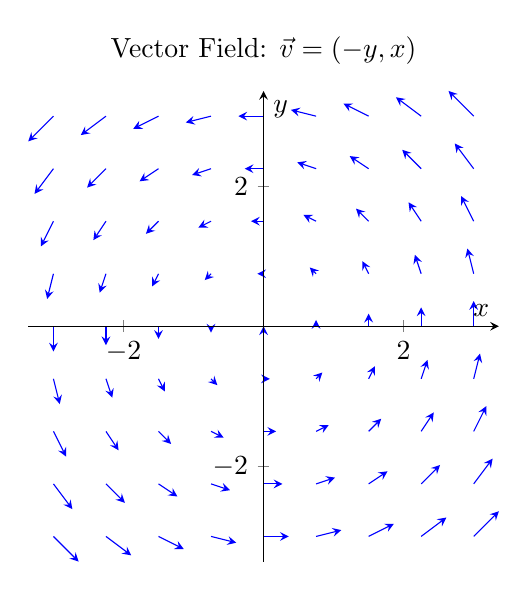
\begin{tikzpicture}
\begin{axis}[
    title={Vector Field: $\vec{v}=(-y,x)$},
    domain=-3:3,
    y domain=-3:3,
    view={0}{90},
    axis lines=middle,
    xlabel={$x$},
    ylabel={$y$},
    samples=9,
    scale=1.05,
    axis equal image
]
\addplot3 [
    blue,
    -stealth,
    quiver={
        u={-y},
        v={x},
        scale arrows=0.12
    }
] (x,y,0);
\end{axis}
\end{tikzpicture}
\end{center}

\subsubsection*{Trajectories}
A \textbf{trajectory} is the actual path followed by a particle moving according to a vector field. If the vector field gives the local velocity, the trajectory is the curve obtained by following that velocity over time.

For the rotational field above, trajectories are circles centered at the origin. The arrows tell the particle how to move at each instant; the trajectory shows the complete journey.

\begin{center}
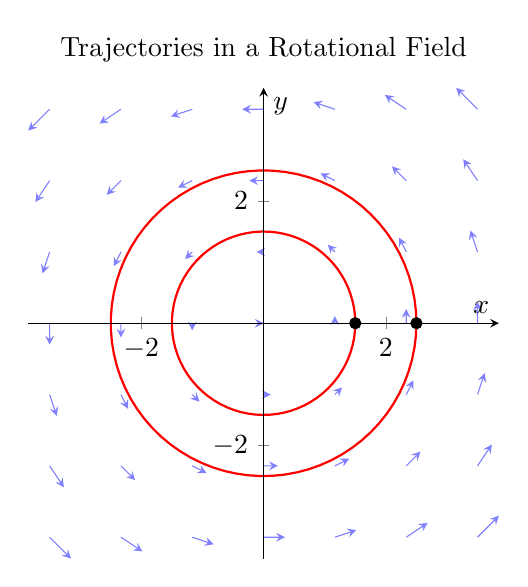
\begin{tikzpicture}
\begin{axis}[
    title={Trajectories in a Rotational Field},
    domain=-3.5:3.5,
    y domain=-3.5:3.5,
    view={0}{90},
    axis lines=middle,
    xlabel={$x$},
    ylabel={$y$},
    samples=7,
    scale=1.05,
    axis equal image
]
\addplot3 [
    blue!50!white,
    -stealth,
    quiver={
        u={-y},
        v={x},
        scale arrows=0.1
    }
] (x,y,0);
\addplot [red, thick, domain=0:360, samples=80] ({1.5*cos(x)}, {1.5*sin(x)});
\addplot [red, thick, domain=0:360, samples=80] ({2.5*cos(x)}, {2.5*sin(x)});
\addplot [only marks, mark=*, mark size=2pt, black] coordinates {(1.5,0) (2.5,0)};
\end{axis}
\end{tikzpicture}
\end{center}

\subsubsection*{Why this matters}
\begin{itemize}[leftmargin=*]
  \item Slope fields describe first-order scalar equations such as $\dfrac{dy}{dx}=f(x,y)$.
  \item Vector fields naturally describe systems of equations and particle motion.
  \item Trajectories turn a local rule into a global picture of motion.
\end{itemize}
